\documentclass[11pt,graphicx,caption,rotating]{article}
\textheight=24cm
\textwidth=18cm
\topmargin=-2cm
\oddsidemargin=0cm
%\usepackage[utf8x]{inputenc}
\usepackage[latin1]{inputenc}
\usepackage[activeacute,spanish]{babel}
\usepackage{amssymb,amsfonts}
\usepackage[tbtags]{amsmath}
\usepackage{pict2e}
\usepackage{ucs}
\usepackage{float}
\usepackage[all]{xy}
\usepackage{graphics,graphicx,color,colortbl}
\usepackage{times}
\usepackage{subfigure}
\usepackage{wrapfig}
\usepackage{multicol}
\usepackage{cite}
\usepackage{url}
\usepackage[tbtags]{amsmath}
\usepackage{amsmath,amssymb,amsfonts,amsbsy}
\usepackage{bm}
\usepackage{algorithm}
\usepackage{algorithmic}
\usepackage[centerlast, small]{caption}
\usepackage[colorlinks=true, citecolor=black, linkcolor=black, urlcolor=black,breaklinks=true]{hyperref}
\hyphenation{ele-men-tos he-rra-mi-en-ta cons-tru-yen trans-fe-ren-ci-a pro-pu-es-tas si-mu-lar vi-sua-li-za-cion}

\begin{document}
\title{\textbf{Thin Film Transistor TFT}}
\author{David Ricardo Mart�nez Hern�ndez \textbf{C�digo}:$261931$}
\date{}
\maketitle

\section{Caracter�sticas}
\noindent
Es un tipo especial de transistor de efecto campo que se fabrica depositando finas pel�culas de silicio activo sobre contactos met�licos y una capa de material diel�ctrico.

\section{Fabricaci�n}
\noindent
Se pueden fabricar con una gran variedad de materiales semiconductores. El m�s com�n es el silicio. Las caracter�sticas del TFT basado en el silicio depende de su estado cristalino. Esto es, que la capa de semiconductor puede ser silicio amorfo, silicio microcristalino, o puede haber sido templado en un polisilicio.
Otros materiales que pueden ser usados como semiconductores en TFTs son el seleniuro de cadmio $(CdSe)$ y �xidos de metal como el �xido de zinc.\cite{page1}\\
Usando semiconductores y electrodos transparentes, como el indio-�xido de esta�o (ITO), los dispositivos TFT pueden hacerse completamente transparentes\cite{page1}.\\
El proceso de deposici�n  es realizado a temperaturas relativamente bajas. Se utiliza la deposici�n qu�mica de vapor y la deposici�n f�sica de vapor. Adem�s, la primera soluci�n de procesado TFT transparente (TTFTs), sobre la base de �xido de zinc, fue anunciado en 2003 por investigadores de la Oregon State University\cite{page1}.\\
El laboratorio portugu�s CENIMAT en la Universidade Nova de Lisboa ha producido el primer TFT completamente transparente a temperatura ambiente. CENIMAT tambi�n desarroll� el primer transistor de papel, que puede conducir a aplicaciones tales como revistas y p�ginas de revistas con im�genes en movimiento.\cite{page1}

\begin{figure}[H]
  \centering
    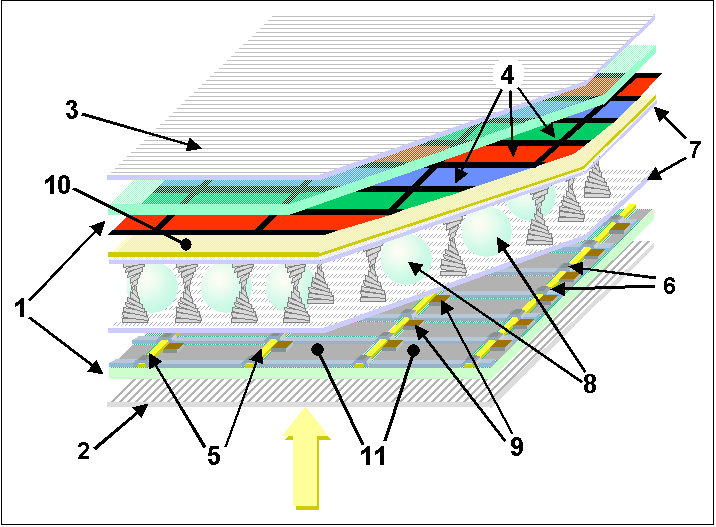
\includegraphics[scale=0.45]{image.png}
      \caption{Matriz de una pantalla TFT (Tomado de \cite{page1}).}
  \label{fig1}
\end{figure}
\noindent
\begin{enumerate}
 \item[1] Placa de vidrio. 
 \item[2-3] Polarizaci�n horizontal y vertical.
 \item[4] Mascara de color RGB.
 \item[5-6] L�nea de comando horizontal y vertical.
 \item[7] Resistente capa de pol�mero.
 \item[8] Separadores
 \item[9] Thin film transistors.
 \item[10] Electrodo frontal.
 \item[11] Electrodos traseros
\end{enumerate}

\section{Aplicaciones}
\noindent
La mejor aplicaci�n actual son\cite{page1}:
\begin{itemize}
 \item Las pantallas TFT LCDs, una implementaci�n de la tecnolog�a de pantalla de cristal l�quido. Los transistores est�n integrados en el propio panel, lo que reduce la diafon�a entre p�xeles y mejorar la estabilidad de la imagen.
 \item En radiograf�a digital y aplicaciones de radiograf�a general. Un TFT se utiliza tanto en la captura directa e indirecta como base para el receptor de imagen en radiolog�a m�dica.
 \item Las nuevas pantallas AMOLED (Diodo org�nico de emisi�n de luz de matriz activa) tambi�n contienen una capa TFT.
\end{itemize}

\bibliographystyle{ieeetran}
\begin{thebibliography}{99}

\bibitem{page1} Wikipedia, the free encyclopedia. Thin-film transistor. Sitio web ``\url{http://en.wikipedia.org/wiki/Thin-film_transistor}'', visitada el 20 de Enero de 2014.

\bibitem{page2} Kuo, Yue. Thin Film Transistor Technology�Past, Present, and Future. ``\url{http://www.electrochem.org/dl/interface/spr/spr13/spr13_p055_061.pdf}'', visitada el 20 de Enero de 2014.
\end{thebibliography}
\end{document}